\chapter{Описание работы программы}
\label{cha:ch_4}


Программа представляет собой исполняемый пакет (для Unix подобных операционных систем), для ее работы не требуется наличие специализированных программ и библиотек.
\par

После запуска программы пользователю предоставляется выбор: создать новую гексагональную сетку или загрузить. При создании новой сетки, появится диалоговое окно, в котором необходимо задать размерность РТДРП. После этого в главном окне появится графическое представление сетки, которое можно редактировать с помощью нажатия левой клавиши мыши (ЛКМ) для увеличение веса выбранного шестиугольника, или правой клавишей мыши (ПКМ) --- для уменьшение. Есть возможность редактирования сетки при зажатой ЛКМ и ПКМ.
\par

\begin{figure}[h]
\begin{center}
\begin{minipage}[h]{0.47\linewidth}
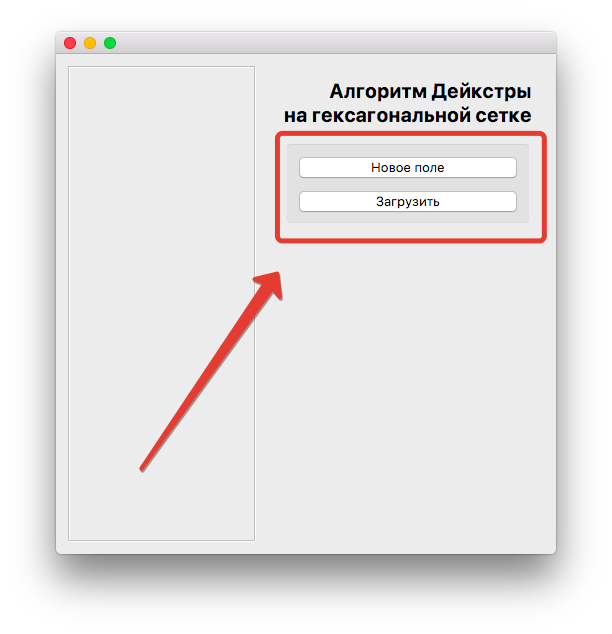
\includegraphics[width=1\linewidth]{inc/img/menuWitCreate}
\caption{Правое боковое меню при отсутствии сетки.} %% подпись к рисунку
\label{axis:cube} %% метка рисунка для ссылки на него
\end{minipage}
\hfill 
\begin{minipage}[h]{0.47\linewidth}
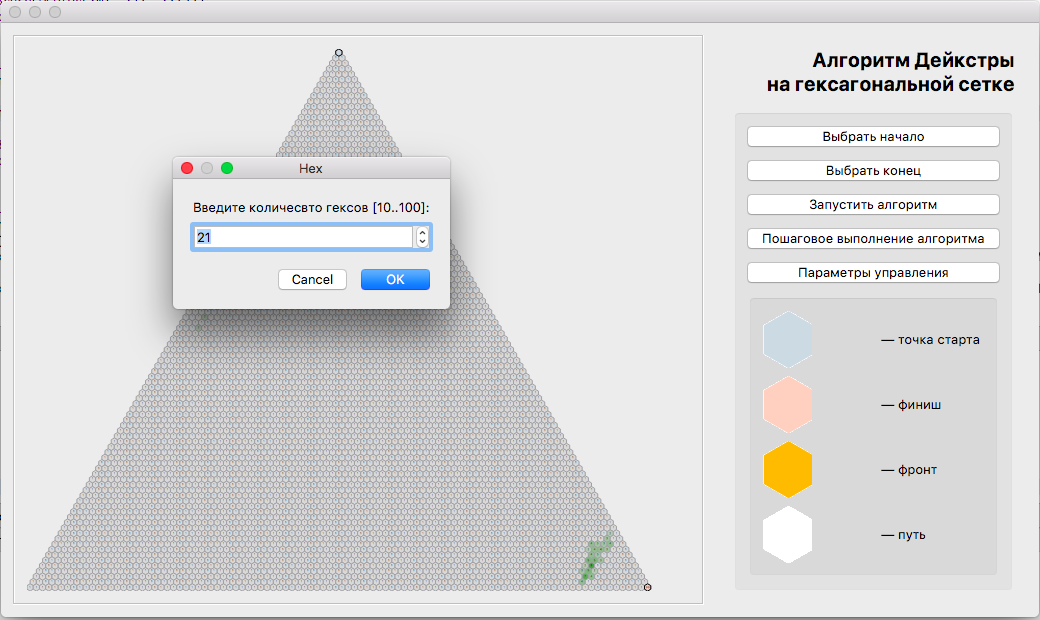
\includegraphics[width=1\linewidth]{inc/img/numOfElems}
\caption{Диалоговое окно, для ввода количества элементов РТДРП.}
\label{axis:axial}
\end{minipage}
\end{center}
\end{figure}

\begin{figure}[h]
\begin{center}
\begin{minipage}[h]{0.47\linewidth}
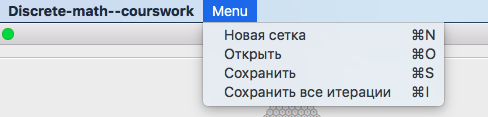
\includegraphics[width=1\linewidth]{inc/img/menu}
\caption{Меню программы.} %% подпись к рисунку
\label{axis:cube} %% метка рисунка для ссылки на него
\end{minipage}
\hfill 
\begin{minipage}[h]{0.47\linewidth}
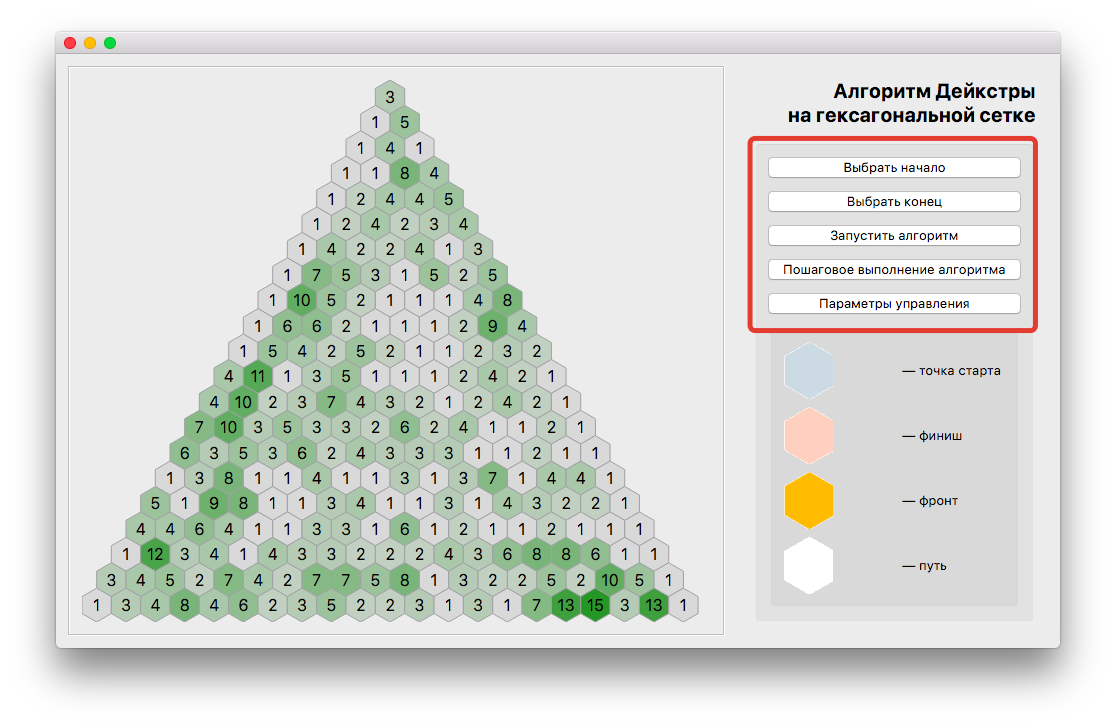
\includegraphics[width=1\linewidth]{inc/img/doSomeThings}
\caption{Правое боковое меню, для выбора действий над сеткой.}
\label{axis:axial}
\end{minipage}
\end{center}
\end{figure}

Перед запуском алгоритма Дейкстры необходимо выбрать начало и конец пути. Для этого в правом боковом меню главного окна необходимо выбрать <<Выбрать начало>>, далее, нажать на желаемый шестиугольник, выбрать в боковом меню <<Выбрать конец>> и нажать на соотвествующий элемент гексагональной сетки. После этого \textbf{возможно} выполнение алгоритма. Для этого необходимо нажать на кнопку в боковом меню <<Запустить алгоритм>>, в результате чего результат сразу отобразится на графическом представлении, или можно выполнить алгоритм пошагово. После каждого нажатия на <<Пошаговое выполнение алгоритма>> на графическое представление будут добавляться шестиугольники, которые добавлены в вектор с длинами кратчайших путей из начала до пройденным элементам. \par

\begin{figure}[h]
\begin{center}
\begin{minipage}[h]{0.47\linewidth}
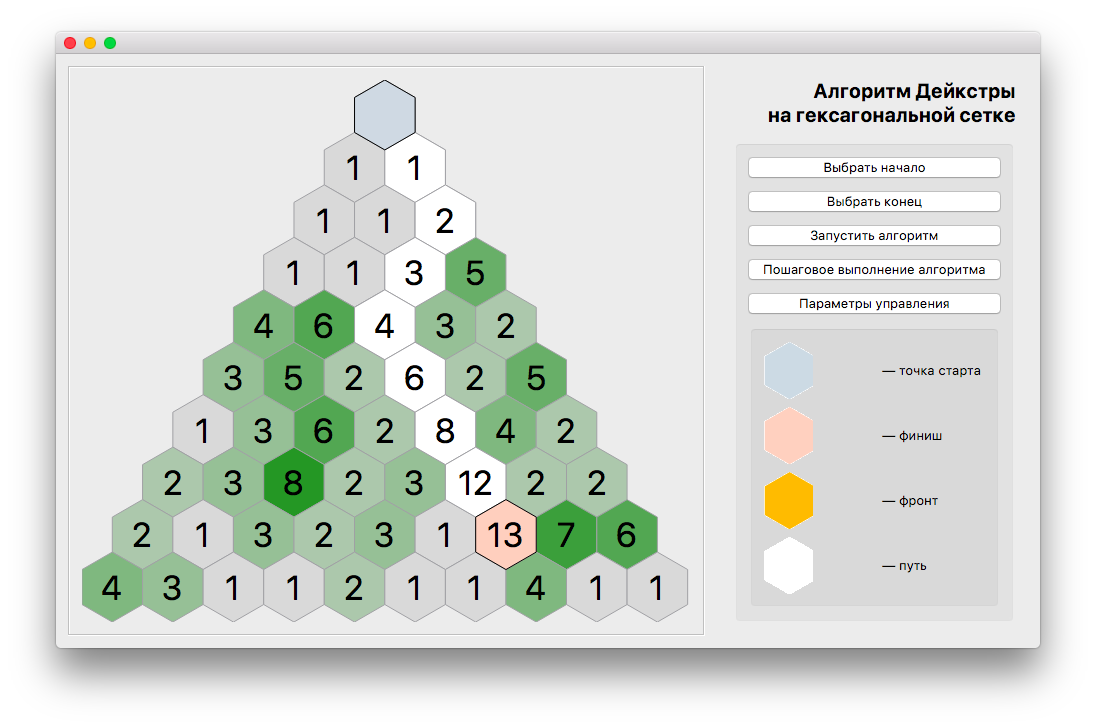
\includegraphics[width=1\linewidth]{inc/img/path}
\caption{Путь.} %% подпись к рисунку
\label{axis:cube} %% метка рисунка для ссылки на него
\end{minipage}
\hfill 
\begin{minipage}[h]{0.47\linewidth}
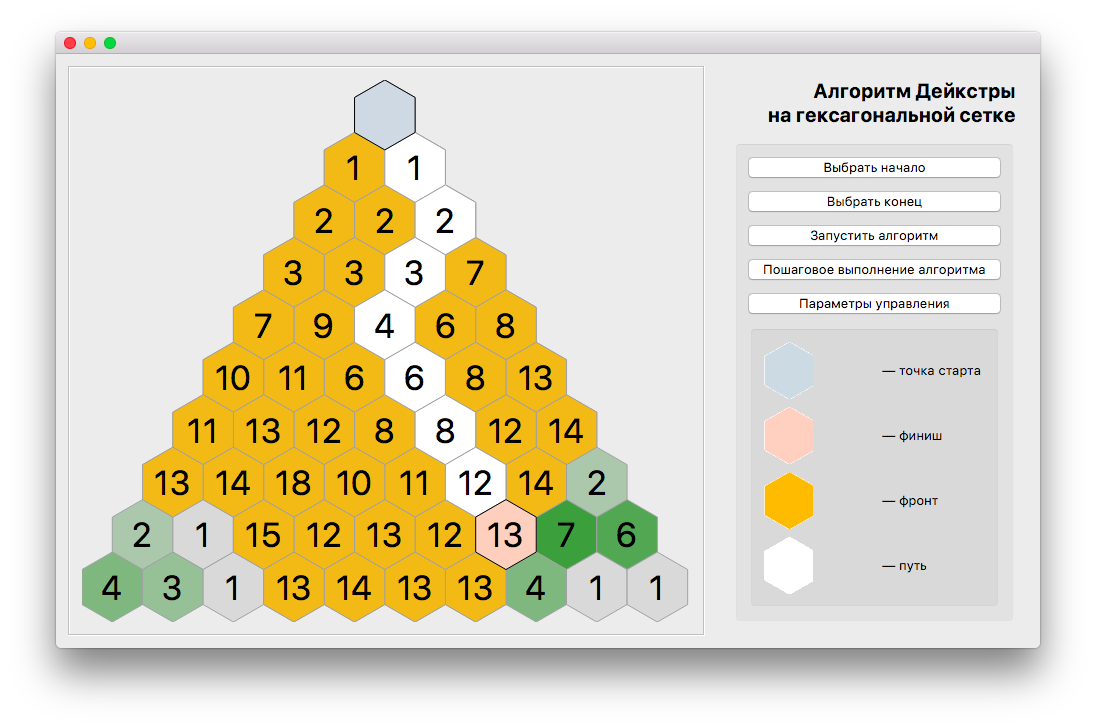
\includegraphics[width=1\linewidth]{inc/img/pathInAlg}
\caption{Путь с итерациями алгоритма.}
\label{axis:axial}
\end{minipage}
\end{center}
\end{figure}
